\subsection{Diboson physics at the LHC}
\label{diboson}

The study of diboson physics is another important test for SM of particle physics in electroweak sector, 
and the Vector Boson Scattering (VBS) is a key process for probing the mechanism of the electroweak symmetry breaking (EWSB).
In the meantime, the non-resonant diboson productions are crucial backgrounds for Higgs studies at the LHC, which make the precise measurement of their cross section becomes very important.

%% ====================================== Diboson productions ========================
\textbf{Diboson productions}

About $90\%$ of diboson productions at hadron collider is from quark-antiquark annihilation,
while others are from gluon initiated process.
Figure~\ref{fig:diboson_fd1} shows the tree-level Feynman diagrams of diboson production.
\begin{figure}[!htb]
  \centering
  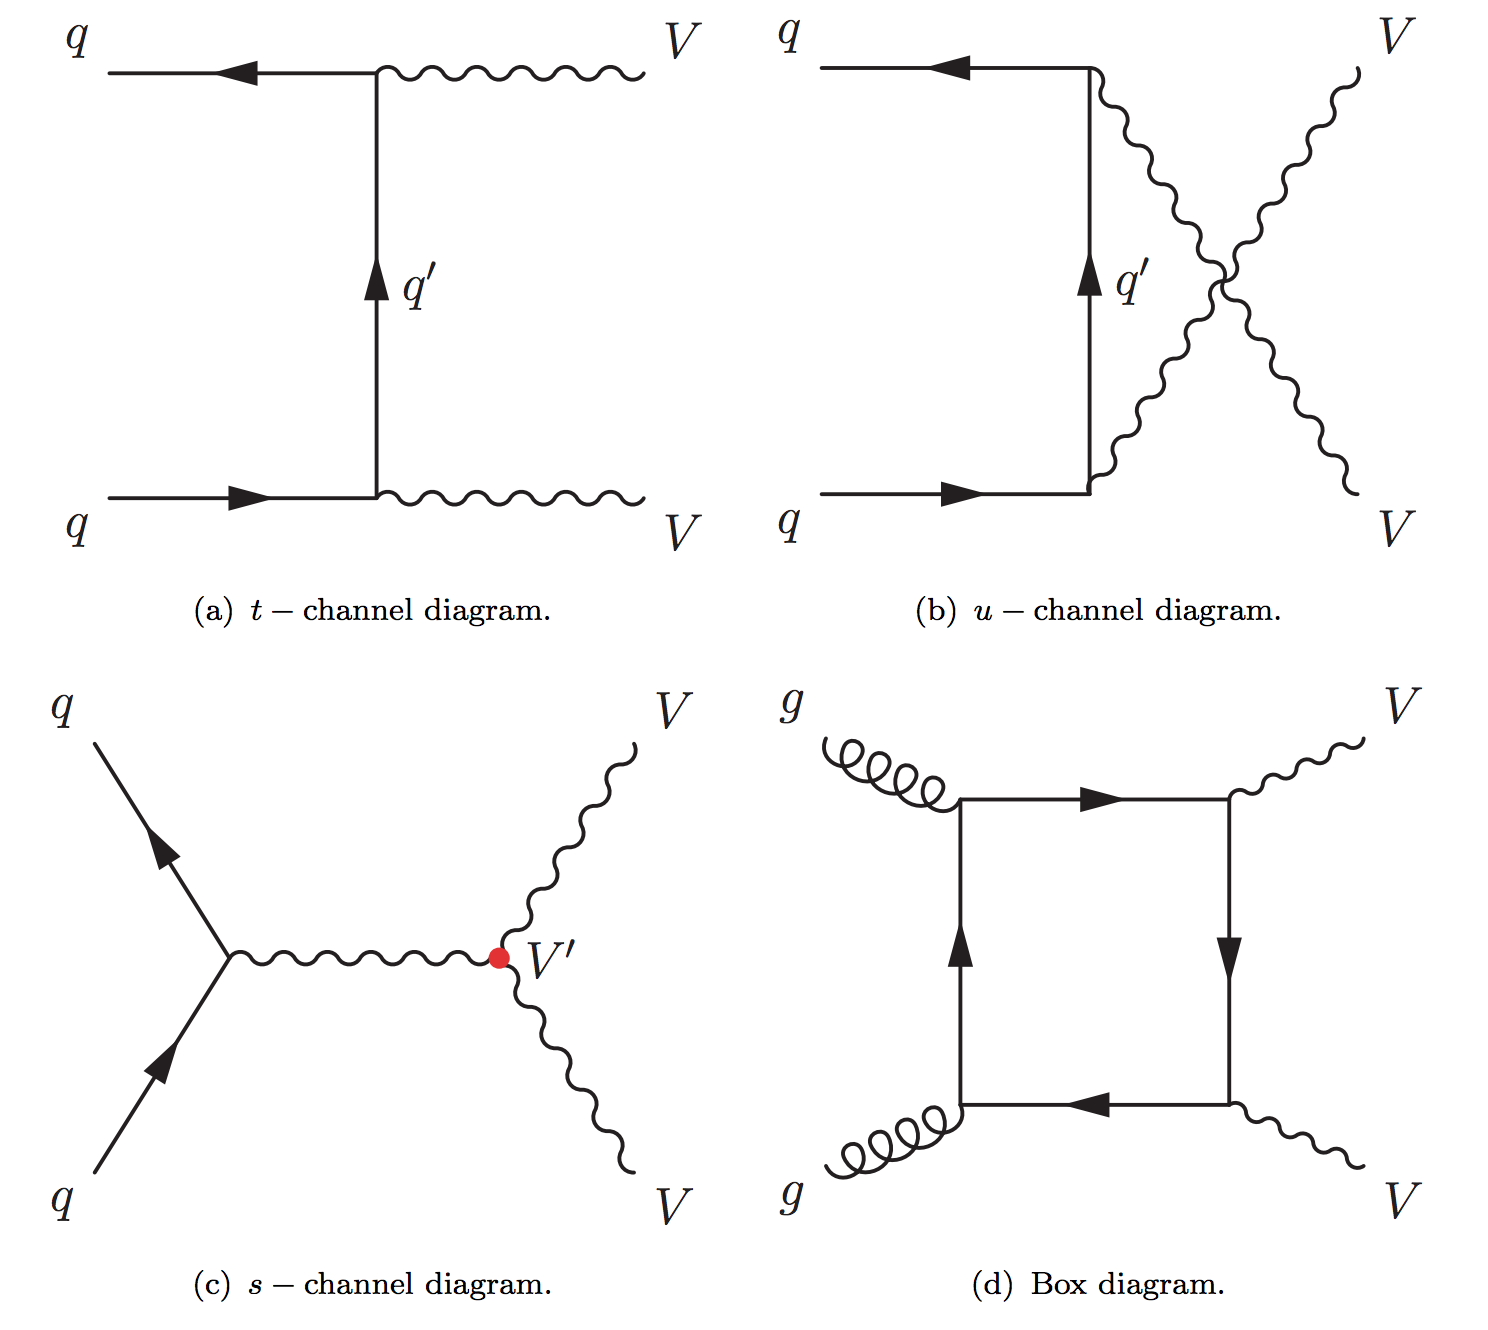
\includegraphics[width=0.7\textwidth]{figures/Theory/diboson_prod_fey.png}
  \caption{The tree-level Feynman diagrams of diboson production at the LHC.}
  \label{fig:diboson_fd1}
\end{figure}
Then figure~\ref{fig:diboson_xs1} illuminates the total production cross-section presented by ATLAS
as a function of centre-of-mass energy $\sqrt{s}$ from 7 to 13~\tev~ for several diboson processes compared 
to some other major processes in hadron collision.
The cross section for diboson processes are calculated at next-to-next leading order (NNLO). 
\begin{figure}[!htb]
  \centering
  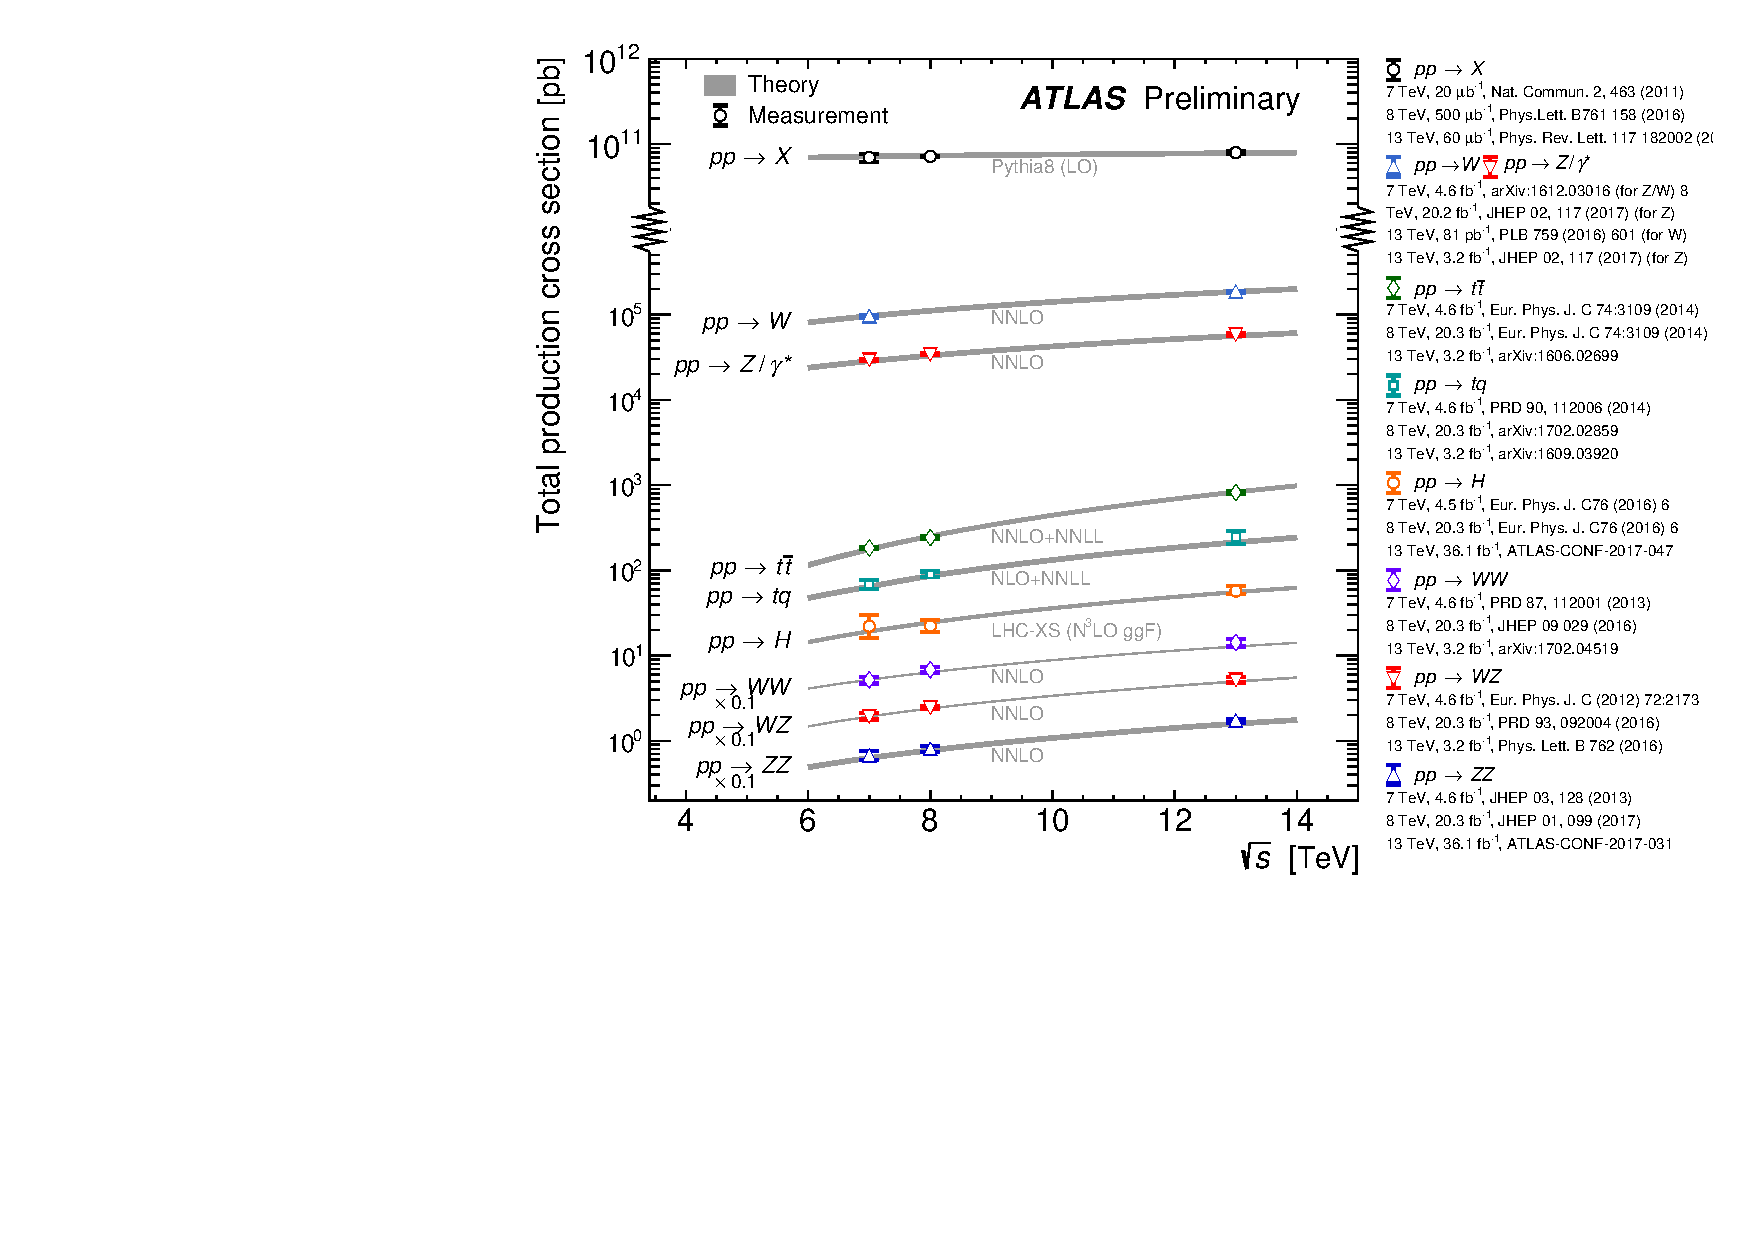
\includegraphics[width=0.7\textwidth]{figures/Theory/ATLAS_n_SMSummary_SqrtS.pdf}
  \caption{Total production cross-section measured by ATLAS as a function of centre-of-mass energy $\sqrt{s}$ from 7 to 13~\tev~ for some selected processes.
	   The measurements of diboson processes are scaled by a factor 0.1 to avoid the overlaps.}
  \label{fig:diboson_xs1}
\end{figure}

%% ======================================= Vector boson scattering ===================
\textbf{Vector boson scattering}

The $SU(2)_{L} \times U(1)_{Y}$ structure in SM predicts self-interactions between electroweak gauge bosons.
Those self-couplings can involve either three or four gauge bosons at a single vertex, known as triple gauge coupling (\textit{TGC}) or
quartic gauge couplings (\textit{QGC}), respectively.
Vector boson scattering (\textit{VBS}) is carried out 
by four electroweak vector bosons, namely $Z$, $W^{\pm}$ and photon $(\gamma)$ as the Feynman diagrams shown in figure~\ref{fig:vbs_fd1}. 
And the vertexes include either those self-interactions
or the interactions with the Higgs boson are described in figure~\ref{fig:vbs_fd2}.
\begin{figure}[!htb]
  \centering
  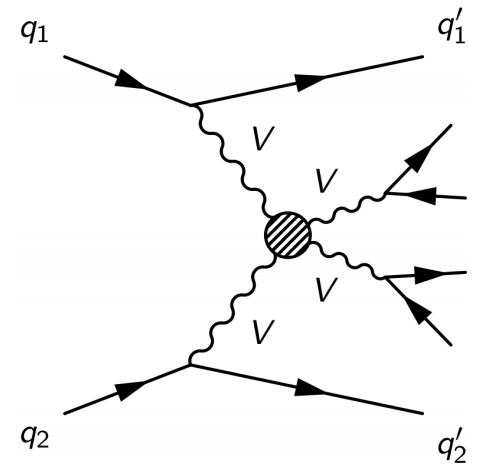
\includegraphics[width=0.4\textwidth]{figures/Theory/VBS.png} 
  \caption{Feynman diagrams of the vector boson scattering process.}
  \label{fig:vbs_fd1}
\end{figure}
\begin{figure}[!htb]
  \centering
  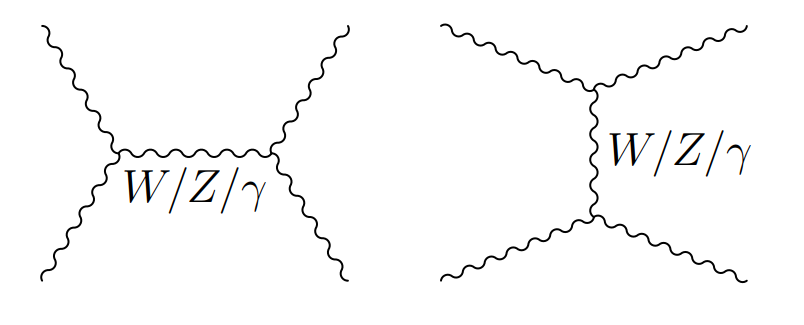
\includegraphics[width=0.6\textwidth]{figures/Theory/vbs_tgc.png} \\
  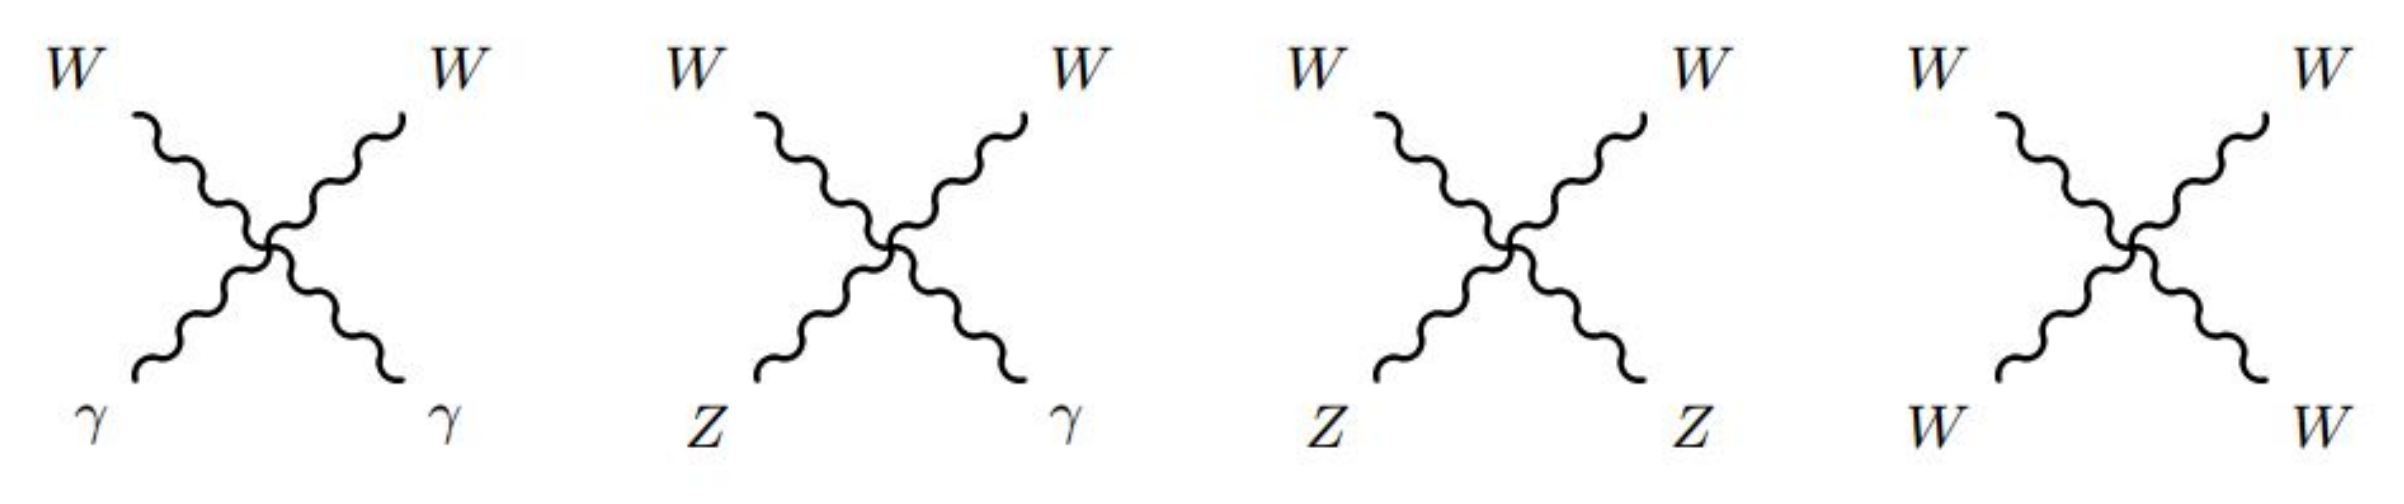
\includegraphics[width=1.0\textwidth]{figures/Theory/vbs_qgc.png} \\
  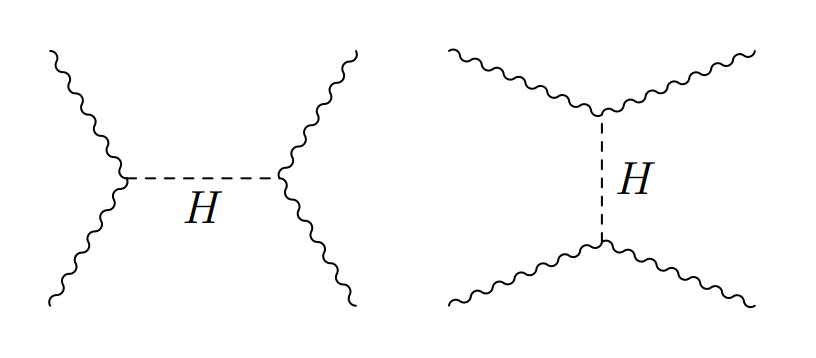
\includegraphics[width=0.6\textwidth]{figures/Theory/vbs_higgs.png} 
  %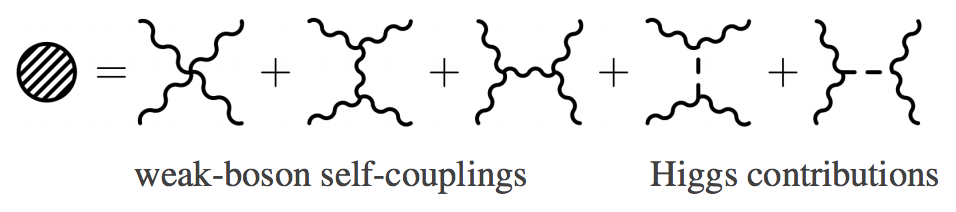
\includegraphics[width=1.0\textwidth]{figures/Theory/VBS_vertex.png}
  \caption{Feynman disgrams of diboson productions with vertexes involving QGC, TGC and Higgs.}
  \label{fig:vbs_fd2}
\end{figure}

The amplitudes of leading-order (LO) VBS can be expressed as\cite{PhysRevD.87.093005}:
\begin{equation} \label{eq:amp_tgc}
\begin{split}
	& {iM}_{TGC}^{s-channel} = -i\frac{g_{1}^{2}}{4m_{W}^{4}}[s(t-u)-3m_{W}^{2}(t-u)] \\
	& {iM}_{TGC}^{t-channel} = -i\frac{g_{1}^{2}}{4m_{W}^{4}}\left[(s-u)t-3m_{W}^{2}(s-u)+\frac{8m_{W}^{2}}{s}u^{2}\right]
\end{split}
\end{equation}
\begin{equation} \label{eq:amp_qgc}
	{iM}_{QGC} = i\frac{g_{1}^{2}}{4m_{W}^{4}}\left[s^{2}+4st+t^{2}-4m_{W}^{2}(s+t)-\frac{8m_{W}^{2}}{s}ut\right]
\end{equation}
\begin{equation} \label{eq:amp_higgs}
\begin{split}
	{iM}_{Higgs} & = -i\frac{C_{\nu}^{2}g_{1}^{2}}{4m_{W}^{2}}\left[\frac{(s-2m_{W}^{2})^{2}}{s-m_{H}^{2}} + \frac{(t-2m_{W}^{2})^{2}}{t-m_{H}^{2}}\right] \\
                     & \simeq -i\frac{C_{\nu}^{2}g_{1}^{2}}{4m_{W}^{2}}(s+t)
\end{split}
\end{equation}
Combining s- and t-channel of TGC in Eq.~\ref{eq:amp_tgc} and the QGC term in Eq.~\ref{eq:amp_qgc}:
\begin{equation} \label{eq:self_coup}
	{iM}_{TGC} + {iM}_{QGC}= i\frac{g_{1}^{2}}{4m_{W}^{2}}(s+t) + {O}((s/m_{W}^{2})^{0})
\end{equation}
In Eq.~\ref{eq:self_coup}, the amplitude grows as a function of centre-of-mass energy ($\sqrt{s}$),
which violates the unitarity in the ~\tev~ region.
Considering the Higgs term in Eq.~\ref{eq:amp_higgs} can perfectly cancel out this growing,
and the remaining term ${O}((s/m_{W}^{2})^{0})$ only depends on the total amplitude in SM.

In conclusion, the Higgs boson acts as ``moderator" to unitarize high-energy longitudinal vector boson scattering
as introducing the Higgs restores the unitarity of total amplitude in high energy region.
